\documentclass[a4paper]{article}
\usepackage[top=1in, bottom=1.25in, left=1.25in, right=1.25in]{geometry}
\usepackage{amsmath}
\usepackage{multicol}
\usepackage{graphicx}
%\RequirePackage{ltxcmds}[2010/12/07]
%opening
\title{Overlap-Save Method}
\author{ }
\date{ }
\begin{document}

\maketitle

In this method the input data sequence is split into blocks of length $N$ samples defined as $N=L+R$. Each block of length $N$ consist of overlapping last $R-1$ samples of the previous block followed by $L$ new samples. Then, the an $N$-point FFT is computed for each data block. Then, the multiplication of $N$-point FFT and the transfer function is performed, followed by IFFT operations to obtain the time-domain block signal. Since the data block is of length $N$, the first $R-1$ samples of the output are corrupt by the aliasing. Thus, these initial samples are then discarded, and only the error-free $N-R$ samples are saved in the output record.
It is important to emphasize that in the beginning of processing the first $R$ samples are set to zero.
In the figure below is illustrated an example of overlap-add method with $R=\frac{N}{2}$ and $L=R$.

\begin{figure}[h]
    \centering
    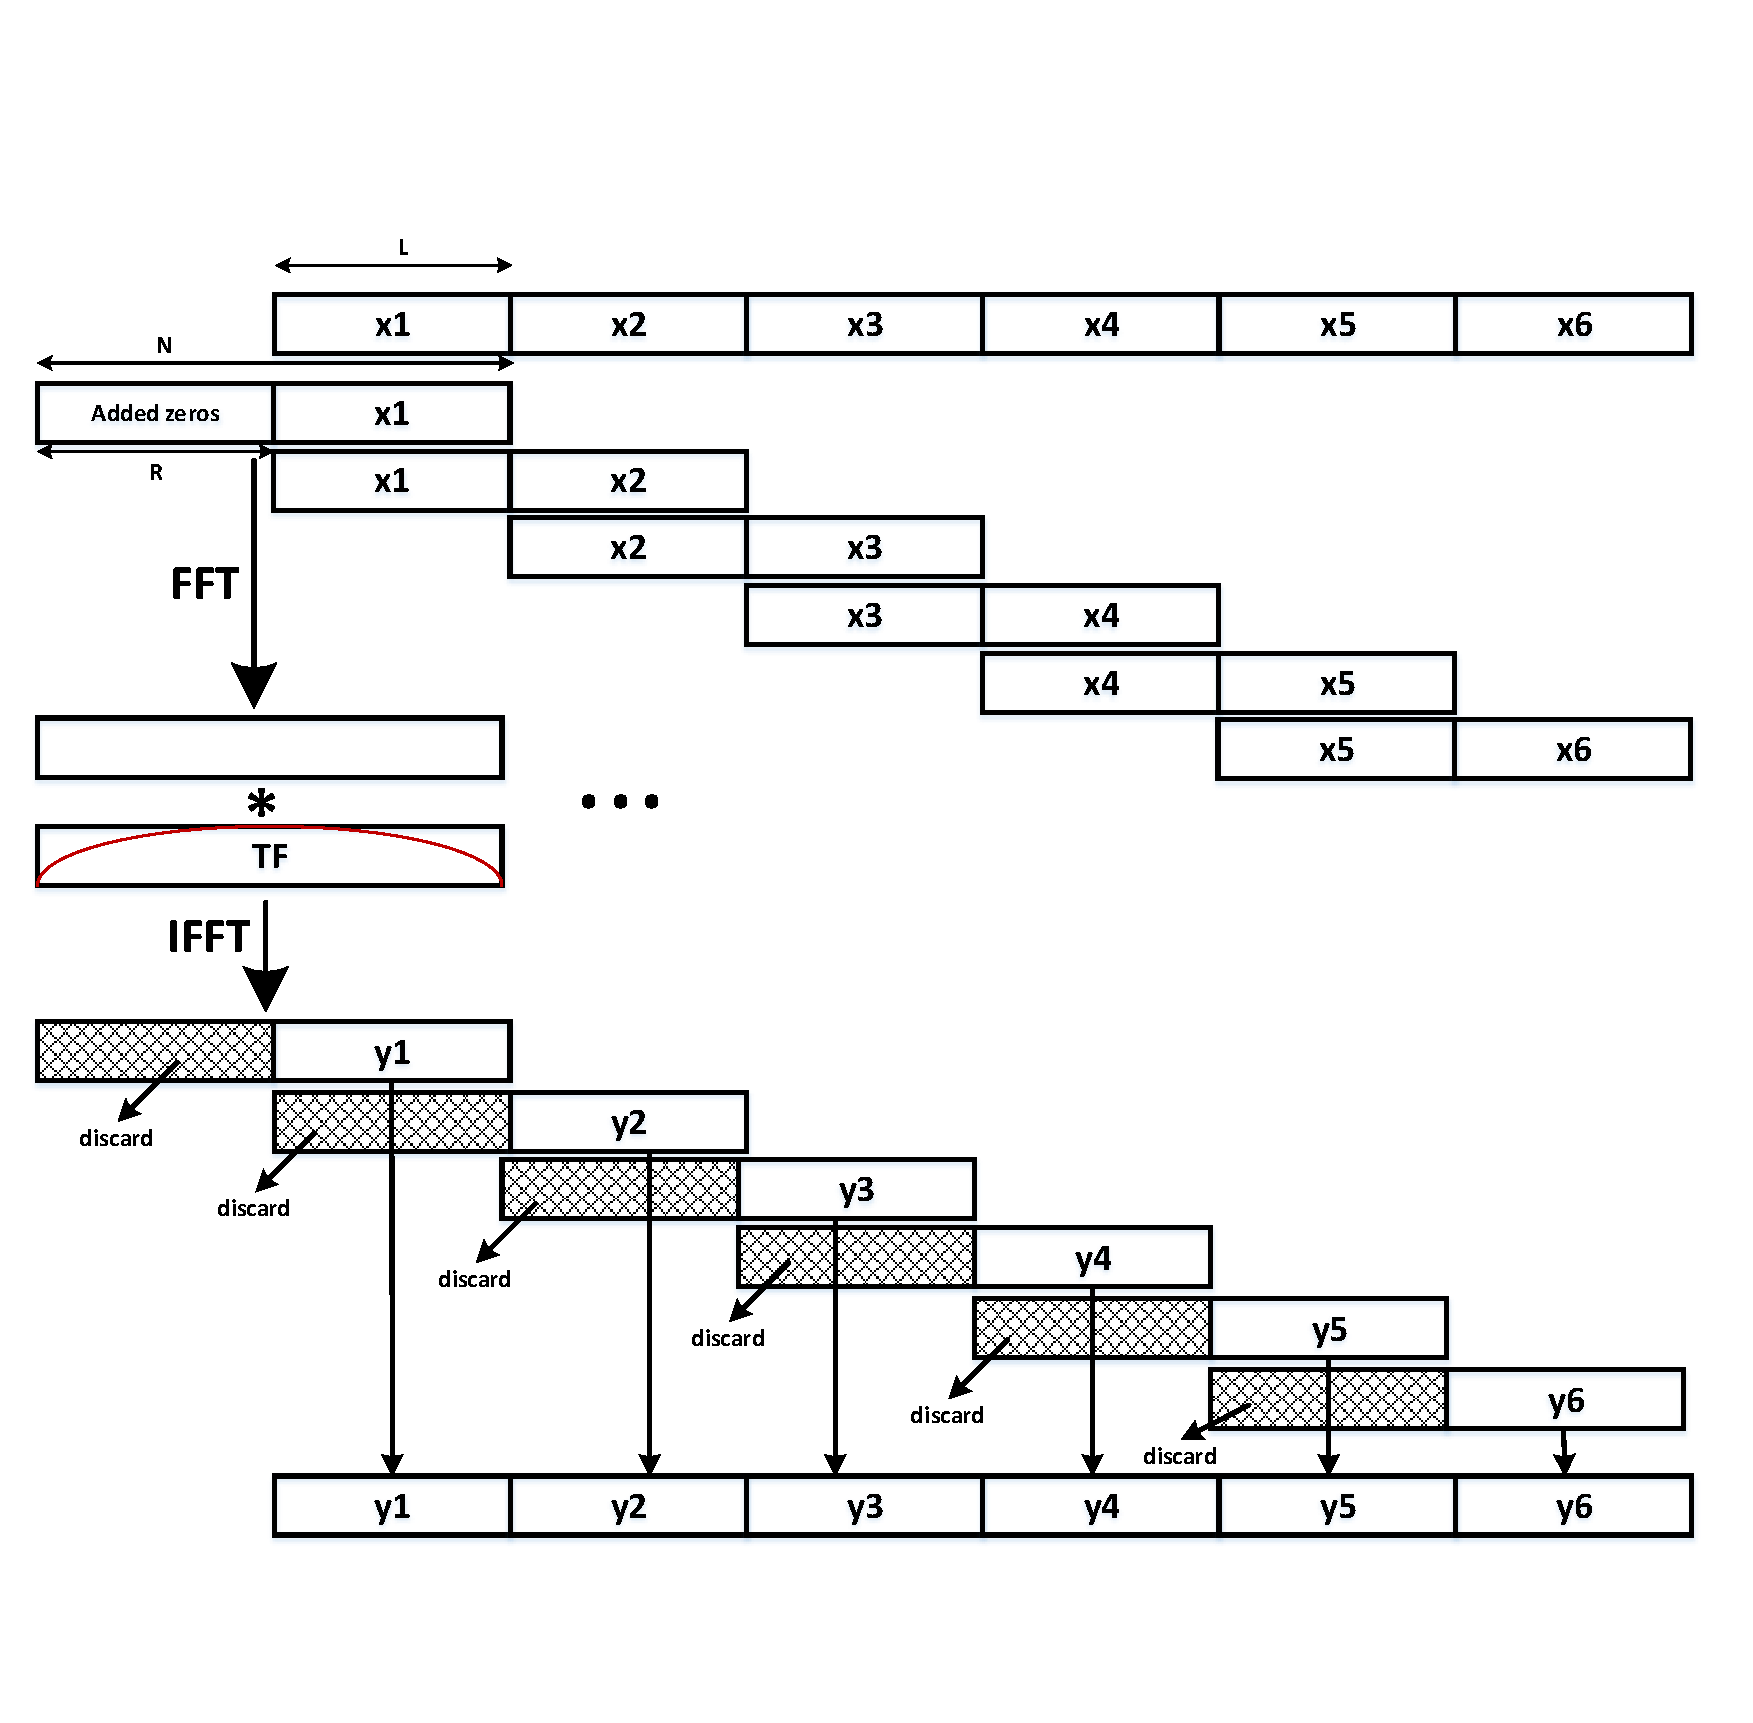
\includegraphics[width=15cm]{overlap-save}
\end{figure}

\end{document} 